%!TEX root = ../../master.tex
\section{Service-Oriented Architecture}
In an enterprise setting, applications often start with a monolithic approach. As the application grows, the need for separation arises. Service-oriented architecture (SOA) gained traction in the beginning of the 00s as organizations started to adopt the new paradigm of online business. The drivers for adopting SOA was, among others, the challenges IT executives were facing of \textit{"cutting costs and maximizing the utilization of existing technology at the same time continuously striving to serve customers better, be more competitive, and be more responsive to the business's strategic plan"} \cite[p. 18]{endrei2004patterns}. The two main drivers for this type of pressure are the need for \textit{heterogeneity} and the need for \textit{change}. 
Endrei et al describe the characteristics needed: \textit{"In order to alleviate the problems of heterogeneity, interoperability and ever changing requirements, such an architecture should provide a platform for building application services with the following characteristics: Loosely coupled, Location transparent, Protocol independent"}
 \cite[p. 19]{endrei2004patterns}. \\


\noindent In order to address these requirements, \textit{functional} decomposition of applications into services is an important factor. Endrei describes services as:  \textit{"A service is generally implemented as a course-grained, discoverable software entity that exists as a single instance and interacts with applications and other services through a loosely coupled, message-based communication model."} \cite[p. 21]{endrei2004patterns}. \\


\noindent 
Communication between services is done in various ways, but popular choices in the SOA community are by using the \textit{Simple Object Access Protocol (SOAP)} over HTTP or using middleware bus-systems like the \textit{Enterprise Service Bus}. SOAP is a protocol for inter-service communication over HTTP. Each SOAP service is bound to a contract using the \textit{Web Service Definition Langauge (WSDL)\footnote{\url{http://www.w3schools.com/xml/xml_wsdl.asp}}} that adheres to an \textit{XML Schema Definition (XSD)\footnote{\url{http://www.w3schools.com/xml/schema_schema.asp}}}. SOAP messages are rather large because they wrap the message in a \textit{SOAP Envelope}, this envelope has a SOAP Header and SOAP Body. The Enterprise Service Bus, on the other hand, acts as a bus that hides complexity and simplifies access, which basically handles the complex details in the background.
The ESB has been criticized by, among others, Jim Webber, Global Head of Architecture at ThoughtWorks, and Martin Fowler, Chief Scientist at ThoughtWorks, in their talk \textit{Does My Bus Look Big in This?}\footnote{\url{https://www.infoq.com/presentations/soa-without-esb}} from 2008. 

\begin{citat} []
"Except, I don't think ESB is Enterprise Service Bus. I think it is Erroneous Spaghetti Box." - \textbf{Jim Webber, 2008}
\end{citat}

\noindent 
The reason for this criticism is the outsourcing of vital pieces of the architecture into middleware components. Webber describes the branding of \textit{"the ESB as the panacea for all your ills"}. However, for many it was not the promised silverbullet. Newman describes SOA as: \textit{"at its heart is a very sensible idea. However despite many efforts, there is a lack of good consensus about how to do SOA well"} \cite[p. 8]{newman2015building}. In his opinion, \textit{"much of the industry has failed to look holistically enough at the problem and present a compelling alternative to the narrative set out by various vendors in this space"} \cite[p. 8]{newman2015building}. He further states that the problems with SOA consist of problems with communication protocols, vendor middleware, and lack of guidance about service granularity. \\

\noindent
A simplified service oriented architecture is visualized in Figure~\ref{fig:soa}. Opposite the monolithic architecture seen in Figure~\ref{fig:monolithic} the architecture is now transformed into an inter-process architecture. This results in communication over network instead of intra-process method invocations.\\ 


\begin{figure}[H]
    \centering
    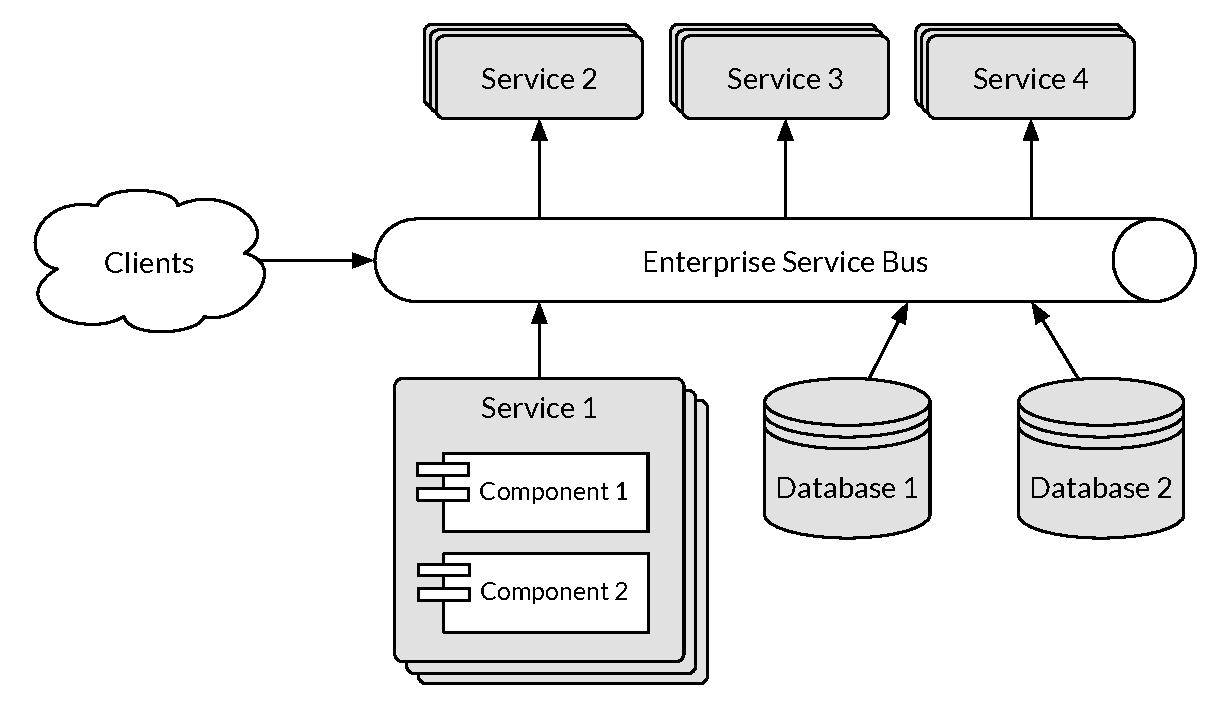
\includegraphics[width=10cm]{figures/service_oriented_architecture}
    \caption{Service-Oriented Architecture (SOA)}
    \label{fig:soa}
\end{figure}


\noindent
The benefits of applying a service-oriented architecture are, among others, independent development of services, independent choice of technology stack for services, increased reuse, more responsive and faster time-to-market.
\noindent
Villamizar describes the shift towards service-oriented architectures and the next step as:
\textit{"To avoid the problems of monolithic applications and take advantage of some of the SOA architecture benefits, the microservice architecture pattern has emerged as a lightweight subset of the SOA architecture pattern"} \cite[p. 584]{villamizar2015evaluating}.